\section{Keys}
\label{sec:keys}

Let $G \in \G$ be a generator for this key derivation scheme.

\Mike{The details for how this $G$ should be derived are fuzzy to me.
Zac describes a method for deriving generators for our Poseidon hash \href{https://hackmd.io/@aztec-network/ryzn3JIu3?type=view\#Deriving-generators-via-hash-to-curve}{here}.
Perhaps this approach can be adopted here, with some domain separator such as $\text{``az\_keys''}$?}

\subsection{Seed}
The $\seed$ is derived out of protocol.
Different hardware \/ software wallets might choose to derive these values in different ways.
A seed is a secret from which all of a user's other keys may be derived.
The $\seed$ can live on an offline device, such as a hardware wallet.\\
\\ 
$\seed \stackrel{\$}{\leftarrow} \mathbb{Z}_{2^{256}}$\\


\subsection{Master keys}

\Todo{correct serialisation of the data into the hash functions.
E.g. conversions from fields to bits, etc.}\\
\\
$\nskm := \shahmac(\text{``az\_nsk\_m''}, \sk) \mod r \in \Fr$, "Master nullifier secret key". App-siloed nullifier secret keys are derived from this. See later for how.\\
\\
$\ivskm := \shahmac(\text{``az\_ivsk\_m''}, \sk) \mod r \in \Fr$, "Master incoming viewing secret key". Used by a recipient to decrypt ciphertexts which are sent to them (hence "incoming").\\
\\
$\ovskm := \shahmac(\text{``az\_ovsk\_m''}, \sk) \mod r \in \Fr$, "Master outgoing viewing secret key". Used by a sender to decrypt ciphertexts which they sent to someone (hence "outgoing"). Depending on some considerations below, this key might also be used when encrypting.\\
\\
$\Npkm := \nskm \cdot G \in \G$, "Master nullifier public key". If we do key rotation (more on this below), a sender of a note will need to include the recipient's $\Npkm$ inside the note, to convey who may nullify the note in future.\\
\\
$\Ivpkm := \ivskm \cdot G \in \G$, "Master incoming viewing public key". Used by a sender to compute symmetric key for encryption.\\
\\
$\Ovpkm := \ovskm \cdot G \in \G$, "Master outgoing viewing public key". Depending on some considerations below, this key might be used when encrypting data to one's self.\\
\\
Note: derivation of the master secret keys doesn't need to happen in a circuit, so $\shahmac$ is acceptable.\\
\\
\Info{Note: the hardware wallet which stores the $\seed$ might not support sha512-hmac.
Be careful using alternative hash functions to derive the randomness of these master keys.
E.g. if the hardware wallet only supports sha256, then it would not be acceptable to compute these master keys as $\text{sha256}(...) \mod r$, since the resulting output (of reducing a 256-bit number modulo $r$) would be biased towards smaller values in $\Fr$.
More uniformity might be achieved by instead computing $\sk$ as $( \text{sha256}(\seed, 1) || \text{sha256}(\seed, 2) ) \mod r$, for example, as a modulo reduction of a 512-bit number is closer to being uniformly distributed in $\Fr$.}




\subsection{Aztec Addresses}

An Aztec address is currently an element of $\Fr$, derived as a \href{https://docs.aztec.network/protocol-specs/addresses-and-keys/address}{hash of lots of information}.\\
\\
Palla \& Khashayar are rocking the boat \href{https://hackmd.io/89n_KZJZQYKsFr0WqaYjDw}{here} with some alternative suggestions; seeking other features. :P.





\subsection{App-siloed keys}

Here are some requirements:
\begin{itemize}
    \item A smart contract (i.e. a circuit) must not be given (or be able to derive from other secrets that they're given) a user's master secret keys.
    \item 3rd-party circuits (which prove things about stuff that happened on-chain) must not be given (or be able to derive from other secrets that they're given) a user's master secret keys.
    \item Users might wish to share certain secret keys with 3rd parties that they trust. But they would \textit{really} need to trust the 3rd party.
\end{itemize}






\subsubsection{Do we even want / need app-siloed viewing keys?}\hfill\\
\\
Note: we definitely need app-siloed \textit{nullifier} keys.\\
\\
\Info{Please see \href{https://hackmd.io/SHRWdRhXRqea7SSjvm7q_g\#Siloed-viewing-keys}{here} for a very detailed discussion around siloing of viewing keys.\\
Tl;dr, there's a blue blox at the bottom of that section that suggests that we should recommend to most app developers that they use master viewing keys in their apps.
They would still need app-siloed nullifier keys.\\
Advanced users can still app-siloe their viewing keys - particularly if the inconveniences of hardened viewing keys are acceptable for their use case.\\
Please do read that linked hackmd section, though (maybe after reading the rest of this doc) - it's quite thorough.}\\
\\
An app still has the option of implementing its own key siloing scheme.
We explore some schemes below.
But it's likely that we'll recommend that basic apps use master viewing keys.



\subsubsection{App-siloed incoming viewing keys}


\subsubsubsection{Non-hardened derivation}\hfill\\
\\
Non-hardened key derivation (named after the similar derivation scheme of non-hardened BIP32 keys) at first appeared to be quite useful scheme for incoming viewing keys.
This scheme has the nice property that a \textit{sender} could derive the app-siloed public key (aka "child" public key) of a recipient, knowing just the recipient's master public key, and without any further interaction with the recipient.

However, if someone learns the child secret key, they can use it to derive the master secret key.
In our setting, that isn't very helpful.
The main motivation for siloing keys was to be able to safely give app-siloed keys to 3rd parties or app circuits without leaking activity across other apps.
If a malicious app or an auditor is fed a child secret key, they could use it to derive the master secret key and hence all activity.
There are ways to avoid divulging a child secret key (be it to a circuit or to an auditor), through the schorr protocol or the chaum-pedersen protocol (or even through snarks if you wanted to use a hammer to crack a nut), but if using such protocols to prove knowledge of secret keys, then why not just use the master keys for that purpose?\\
\\
We've concluded that non-hardened keys aren't of use in Aztec.
For posterity, we explain non-hardened key derivation (without rigour or review) in the appendix.





\subsubsubsection{Hardened derivation}\hfill\\
\\
Hardened keys are safer than non-hardened keys, because the master secret key can't be derived from a child secret key.
But they're also less convenient for usage as incoming viewing keys.
Blockchains often seek a nice property that a sender can send a recipient funds, given only an address (and maybe some master public keys) even if the recipient has never interacted with the chain before. (This property is commonly referred to as "counterfactual addresses").
That's why non-hardened bip32, or Identity-based encryption (IBE) were such nice ideas: because they enabled this property.
Hardened BIP32 requires the \textit{recipient} to derive the app-siloed public key and actively share it with potential senders.
They might share it off-chain, or they might share it by creating a transaction which broadcasts or stores the app-siloed public key.

But the recipient might end up in a catch-22, where they need to transact in order to broadcast their app-siloed public key so that they can be paid, but they can't transact because they don't have funds yet, but they can't receive funds to pay for a transaction because they haven't broadcast their app-siloed public key, but they can't transact because they don't have funds yet...\\
\\
The recipient (and not any sender) can derive their own hardened app-siloed incoming viewing public key via:\\
\\
$\ivskapp := \poseidon("az\_ivpk\_app\_hardened", \appaddress, \ivskm)  \in \Fr$\\
\\
$\Ivpkapp = \ivskapp \cdot G \in \G$\\
\\
\Info{Note that this derivation deviates significantly from BIP32 hardened keys, by making huge simplifications.
It's almost unrecognisable, but the name "hardened" has stuck with us, because it conveys that only the owner of the secret keys can derive the hardened child public key.}\\
\\
\Question{Is this scheme secure?}

\subsubsubsection{Non-hardened, hardened, IBE, or master?}\hfill\\
\\
It depends, and apps can choose!
\\
IBE is probably too slow to prove or expensive to broadcast.
It also results in ciphertexts which are larger than AES ciphertexts, which would make IBE logs distinguishable (to observers) from non-IBE logs.
In the interest of maintaining good privacy sets, we're not inclined to recommend this approach.\\
\\
The above-described catch-22 of using hardened incoming viewing keys might make them unusable for many apps.
But apps that assume a user already has funds on Aztec could make use of these keys, by requiring a would-be recipient to register their keys with the app up-front.
And if an app enables off-chain interaction between a recipient and sender, then the would-be recipient can interact with a sender and provide the app-siloed public key off-chain.\\
\\
Non-hardened key derivation is cool, but has these downsides:
\begin{itemize}
    \item If an app wants to prove attempted decryption, then either:
    \begin{itemize}
        \item The app would need to be given $\ivskappnonhardened$, which MUST NOT happen (because that would leak $ivskm$) - the PXE MUST prevent injection of $\ivskappnonhardened$ into circuits; or
        \item The user would need to prove knowledge of $\ivskappnonhardened$, and prove correct derivation of the symmetric key of the ciphertext. See later for how this can be done. This process would be quite slow though, so probably not practical for trial-decrypting the entire blockchain's history. 
    \end{itemize} 
    \item If you want to share $\ivskappnonhardened$ with a trusted 3rd party, you're effectively also sharing your \textit{master} secret key with them.
    \begin{itemize}
        \item Another approach would be to prove correct derivation of a symmetric key, for every (master public key, ephemeral public key, ciphertext) tuple.
    \end{itemize}
    \item An approach to reducing the amount of data to brute-force (when proving attempted decryption) would be to share handshaking shared secrets with that party, enabling the 3rd party to derive the user's tags, and then prove derivation of every symmetric key of every ciphertext that corresponds to those tags, and provide the resulting plaintexts to the 3rd party. This is convoluted, but it does protect the master secret key $\ivskm$.
\end{itemize} 
\noindent
Apps could also just have users use their \textit{master} incoming viewing keypair for encrypting and decrypting, instead of app siloing.
This would give a user less control over what a trusted 3rd party can see, because the 3rd party would be able to see everything with a master viewing secret key.
Note, however, that the trick of proving correct derivation of a symmetric key (as mentioned directly above) is still possible with master keys. See later for how this works.\\
\\
\textbf{We'll likely recommend that app developers use a user's \textit{master} viewing keys within their apps.
Schnorr and Chaum-Pedersen proofs can be used to prove knowledge of master viewing secret keys, and to prove correct derivation of symmetric keys.
If an app can afford the inconvenience of having users interact or register viewing keys, then hardened keys are a good approach.}







\subsubsection{App-siloed nullifier keys}\hfill\\
\\
The requirements for deriving siloed nullifier keys are different from those of siloed incoming viewing keys.
Whilst we were seeking a way for a \textit{sender} to be able to derive a recipient's siloed incoming viewing public key, we don't have this complication when it comes to derivation of siloed nullifier keys.
That's because:
\begin{itemize}
    \item a siloed nullifier \textit{public} key is not useful to us; a sender can just emplace the recipient's \textit{master} $\Npkm$ into notes that he creates for a recipient; and
    \item only the \textit{recipient} needs to derive the app-siloed secret key (of course) in order to derive the nullifier for their notes.
\end{itemize} 
\noindent
\Info{There are two competing approaches at the moment.\\
\\
Approach A requires some key derivation logic in a kernel circuit, which isn't ideal.\\
\\
Approach B enables the key derivation logic to be validated within an app-circuit, which is cleaner, but it could require more constraints because it uses more elliptic curve operations.
It's very difficult to determine which approach is most efficient.\\
\\
Please see \href{https://hackmd.io/@aztec-network/HyqlobuIR?type=view}{here} for further explanation of Approach B (although the maths notation is different from here, so maybe ignore the actual maths in that hackmd and focus on the other stuff), including arguments in favour of Approach B, and a table which attempts to compare the gate counts of the approaches.
We'll also describe approach B below, without the discussion on gate counts.
}\\
\\
\Info{\textbf{We're currently leaning towards Approach B, as it removes logic and concepts from the protocol.}}\\
\\
\Info{Here, $\appaddress \in \Fr$, but there are \href{https://hackmd.io/89n_KZJZQYKsFr0WqaYjDw}{more-recent discussions} that might change the definition and type of an $\appaddress$ in search of other nice properties.
We'll ignore those newer discussions, for now.}

\subsubsubsection{Approach A}\hfill\\
\\
$\nskapp := \poseidon(\text{``az\_nsk\_app''}, \appaddress, \nskm)$\\
\\
The downside to this approach is that we needed to introduce logic inside a "reset kernel circuit" which performed "key validation", because an app circuit is not allowed to be given $\nskm$, whilst a kernel circuit can be trusted with a master secret key.
Introducing this opinionated key derivation logic at the protocol level is unpopular, and might lead to non-obvious constraint inefficiencies (see \href{https://hackmd.io/@aztec-network/HyqlobuIR?type=view}{here}).\\
\\
The logic inside the key validation reset circuit is:\\
\\
\begin{itemize}
    \item Input from app:
    \begin{itemize}
        \item $\Npkm, \nskapp, \appaddress$.
    \end{itemize}
    \item Input injected by the PXE as a witness:
    \begin{itemize}
        \item $\nskm$.
    \end{itemize}
    \item Assert:
    \begin{itemize}
        \item $\Npkm == \nskm \cdot G$
        \item $\nskapp == \poseidon(\text{``az\_nsk\_app''}, \appaddress, \nskm)$ 
    \end{itemize}
\end{itemize}


\subsubsubsection{Approach B}\hfill\\
\\
This is the currently-preferred approach, if the maths is good. Is thie Chaum-Pedersen?\\
\\
In addition to the $G$ generator defined above in the "Master Keys" section, also define generators $\Gsilo, \Gappaddress \in \G$, which are generated with some neat domain separators.\\
\\
Let $\Nskapp \in \G$ be:\\
\\
$\Nskapp := \nskm \cdot \Gsilo + \appaddress \cdot \Gappaddress \in \G$\\
\\
Notice, it's a point, which is kind of weird and inconsistent with the master secret keys' type, but let's continue.\\
\\
Deriving the app-siloed secret key in this algebraic way means that knowledge of $\nskm$ can be proven to the circuit, without passing the secret key \textit{into} the circuit.
Recall: $\nskm$ must never enter an app circuit.\\
\\
Prover $\P$ wants to prove they know $\nskm$ and that they used it to compute $\nskm \cdot \Gsilo$, without revealing $\nskm$:\\
\\
Prover $\P$ does the following, off-chain (outside of a circuit, in typescript-land or c++-land):

\begin{itemize}
    \item Let $A, B \in \G$ be defined as:
    \begin{itemize}
        \item $A := \Npkm := \nskm \cdot G$
        \item $B := \nskm \cdot \Gsilo$
    \end{itemize}
    \item Choose random $\alpha \stackrel{\$}{\leftarrow} \Fr$.
    \item Let $A', B' \in \G$ be defined as:
    \begin{itemize}
        \item $A' := \alpha \cdot G$
        \item $B' := \alpha \cdot \Gsilo$
    \end{itemize}
    \item Compute challenge $c \leftarrow \poseidon(A, B, A', B') \in \Fr$.
    \item Compute $t \leftarrow \alpha - c \cdot \nskm \mod r \in \Fr$.
\end{itemize}

\noindent
$\P$ passes the following as inputs to the circuit:

\begin{itemize}
    \item $A, B, A', B', t$
\end{itemize}

\noindent
Verifier $\V$ (in this case, the circuit) does the following:

\begin{itemize}
    \item Looks-up $\Npkm$ for $\P$'s address, and asserts $A == \Npkm$.
    \item Recomputes challenge $c \leftarrow \poseidon(A, B, A', B') \in \Fr$.
    \item Checks:
    \begin{itemize}
        \item $A' == t \cdot G + c \cdot A$ 
        \item $B' == t \cdot \Gsilo + c \cdot B$ 
    \end{itemize}
\end{itemize}
\noindent
Notice:
\begin{align*}
    A' &== t \cdot G + c \cdot A\\
    => \alpha \cdot G &== (\alpha - c \cdot \nskm) \cdot G + c \cdot (\nskm \cdot G)
\end{align*}
\noindent
This proves that $\P$ knows $\nskm$ and used it in computing $B := \nskm \cdot \Gsilo$.\\
\\
The circuit can then derive $\Nskapp \leftarrow B + \appaddress \cdot \Gappaddress$, which is the whole objective of this section.\\
\\
A nullifier for a note can then be derived as something like:\\
\\
$\text{nullifier} = \poseidon(\text{"az\_nullifier"}, \Nskapp)$
\\
See later for more rigour around deriving a nullifier properly.\\
\\
\Question{Is this secure?}
\Question{Can we reduce the number of scalar multiplications in the "Checks" that $\V$ does, by combining the checks as:\\
\\
$A' + B' == t \cdot (G + \Gsilo) + c \cdot (A + B)$\\
\\
? Or does that give the prover freedom to construct malicious $B$, by fiddling $A', B'$? 
}




\subsubsection{App-siloed outgoing viewing keys}\hfill\\

The requirements for deriving siloed \textit{outgoing} viewing keys are different from those of siloed \textit{incoming} viewing keys.
Whilst we were seeking a way for a \textit{someone else} to be able to derive a user's siloed incoming viewing public key, we don't have this complication when it comes to derivation of siloed outgoing viewing public keys.
That's because:
\begin{itemize}
    \item only the \textit{owner} of an app-siloed outgoing viewing keypair ever needs to derive outgoing ciphertexts. There's never a case where \textit{someone else} needs to derive a user's app-siloed outgoing viewing keypair.
\end{itemize}
\noindent
Similarly to the preceding section on deriving nullifier keys, there are two possible approaches to deriving app-siloed outgoing viewing keys.
The approaches are basically the same as above, just with different letters, and we're leaning towards Approach B.
Here's a more brief summary.
The method for proving knowledge of $\ovskm$\\
\\
\subsubsubsection{Approach A}\hfill\\
\\
$\ovskapp := \poseidon(\text{``az\_ovsk\_app''}, \appaddress, \ovskm)$\\
\\
The downside to this approach is that we needed to introduce logic inside a "reset kernel circuit" which performed "key validation".
See the above nullifier section for how that would work.

\subsubsubsection{Approach B}\hfill\\
In addition to the $G$ generator defined above in the "Master Keys" section, also define generators $\Gsilo, \Gappaddress \in \G$, which are generated with some neat domain separators.\\
\\
Let $\Ovskapp \in \G$ be:\\
\\
$\Ovskapp := \ovskm \cdot \Gsilo + \appaddress \cdot \Gappaddress \in \G$\\
\\
Notice, it's a point, which is kind of weird and inconsistent with the master secret keys' type, but let's continue.\\
\\
Deriving the app-siloed secret key in this algebraic way means that knowledge of $\ovskm$ can be proven to the circuit, without passing the secret key \textit{into} the circuit.
Recall: $\ovskm$ must never enter an app circuit.\\
\\
For the prover $\P$ to prove they know $\ovskm$ and that they used it to compute $\ovskm \cdot \Gsilo$, without revealing $\ovskm$, see the above section on nullifier keys.




\subsection{Key rotation}

\Info{See a brief list of pros \& cons of key rotation \href{https://hackmd.io/SHRWdRhXRqea7SSjvm7q_g\#Key-Rotation}{here}.}\\
\\
\Info{Current consensus seems to be to keep "key rotation" as a feature.
It does cost constraints though, when reading the current keys, and this extra constraint cost might be enough for people to eventually want to scrap key rotation.}\\
\\
How does key rotation work?\\
\\
Very briefly:\\
\\
A user registers their master public keys $\Npkm, \Ivpkm, \Ovpkm$ against their $\address$ in a Key Registry contract which is designed, built, and deployed by the protocol devs.
The idea would be that all users submit their public keys to this registry, and all apps read from this registry. An app would query the public keys for a given address.\\
\\
Since the keys are being stored in Aztec's public data tree, reading the keys of a user results in 40+ poseidon hashes.
A poseidon hash of 2 fields is approx. 80 constraints.
These extra constraints is the main source of controversy.\\
\\
To rotate their keys, a user would simply make a call to the Key Registry from their account contract, specifying the new set of public keys.\\
\\
Note that this existence of key rotation impacts how apps must create notes.
Previously (pre key rotation), a note on Aztec contained the \textit{address} of a user.
But with key rotation that results in double spends.
A user could spend a note with a nullifier = hash(note, nsk\_1).
They could then rotate their nullifier public key, and create an equally-valid alternative nullifier for the same note as nullifier = hash(note, nsk\_2).
This would be bad.
To combat this, the user identifier contained within a note must be their Npk.
This way, if a user rotates their keys, the Npk inside the note doesn't change, so there's only ever one valid nullifier.

\Patrick{(from the big diagram): If the nullifier key becomes part of the note-hash preimage, then one would have to keep that nullifier key as long as the note has not been spent.
That defies key rotation, correct?}

\Mike{It's certainly not ideal.
As you say, it means rotation of keys does not enable you to spend your pre-existing notes if you lost your old keys.
Key rotation also doesn't save your pre-existing notes from an attacker who learned your old keys: the attacker won't be able to spend your pre-existing notes (because they would also need to know your account contract's auth key), but they'd be able to see when you spend your pre-existing notes.}\\
\\
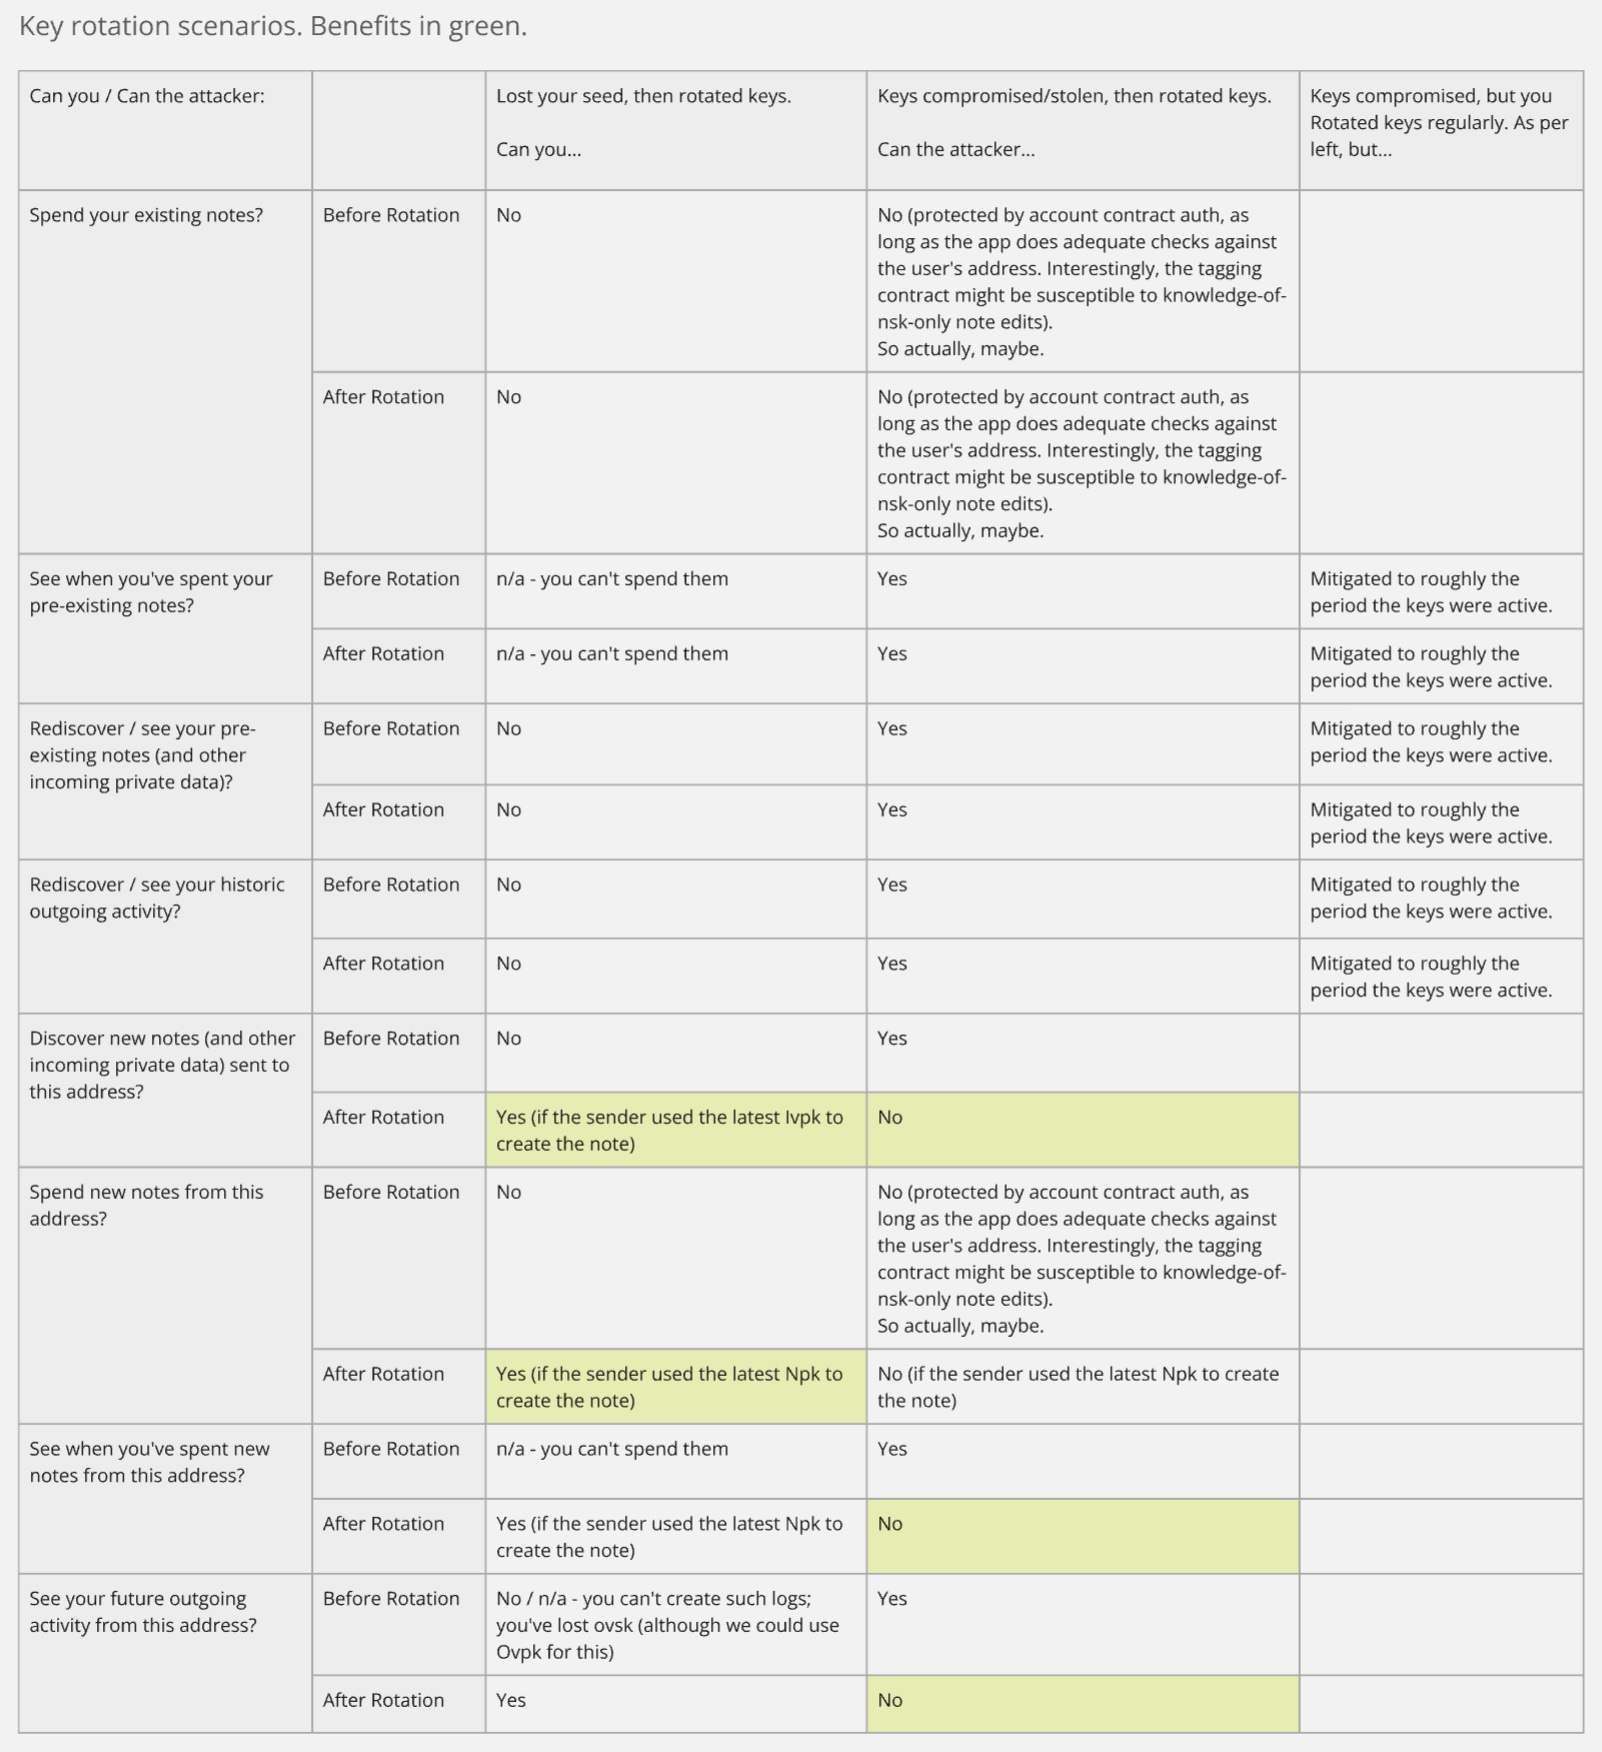
\includegraphics[scale=0.25]{key_rotation.jpg}